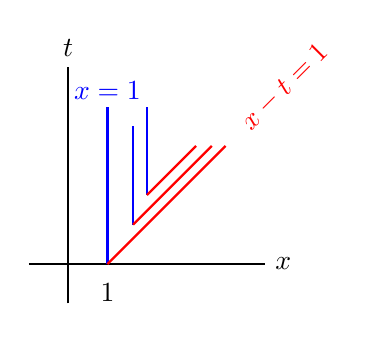
\begin{tikzpicture}[scale=0.5]

\draw[thick] (-1,0)--(5,0) node[right]{$x$};
\draw[thick] (0,-1)--(0,5) node[above]{$t$};

\node[label={below:$1$}] at (1,0) {};

\draw[thick, blue](1,0) -- (1,4) node[pos=1.1]{$x=1$};
\draw[thick, red]  (1,0) -- node[sloped,pos=1.5] {$x-t=1$} (4,3);

\draw[thick, blue](1.65, 1) -- (1.65, 3.5);
\draw[thick, red]  (1.65, 1) -- (3.65, 3);

\draw[thick, blue](2, 1.75) -- (2, 4);
\draw[thick, red]  (2, 1.75) -- (3.25, 3);

\end{tikzpicture}